\section{Reproducibility}
The attenuation coefficients found in the previous section is from the simulated events with given CCDB constants as input.
One way to test the result is to compare the input and the output coefficients. However, the coefficents cannot be directly
compared to one another as different coefficients can define the same exponential form (Eq.~\ref{eq:attn}) reasonably. Therefore, 
the better way of comparison is to compare the exponential forms they define as a function of distance.

\FloatBarrier
\subsection{Without Iteration}
Figure \ref{fig:compGenCalcU} shows the difference of the $y$ values calculated from the generated and calculated coefficients
for a given distance for the U-view. Similar plot for the V- and W-views are shown in Figures~\ref{fig:compGenCalcV} and 
\ref{fig:compGenCalcW} respectively. It can be seen that the coefficients are reproduced within 5\% for longer strips
in each views. The shorter strips are not reproduced that well. One reason is very low number of events in each bin for
short strips.

\begin{figure}[h]
\centering
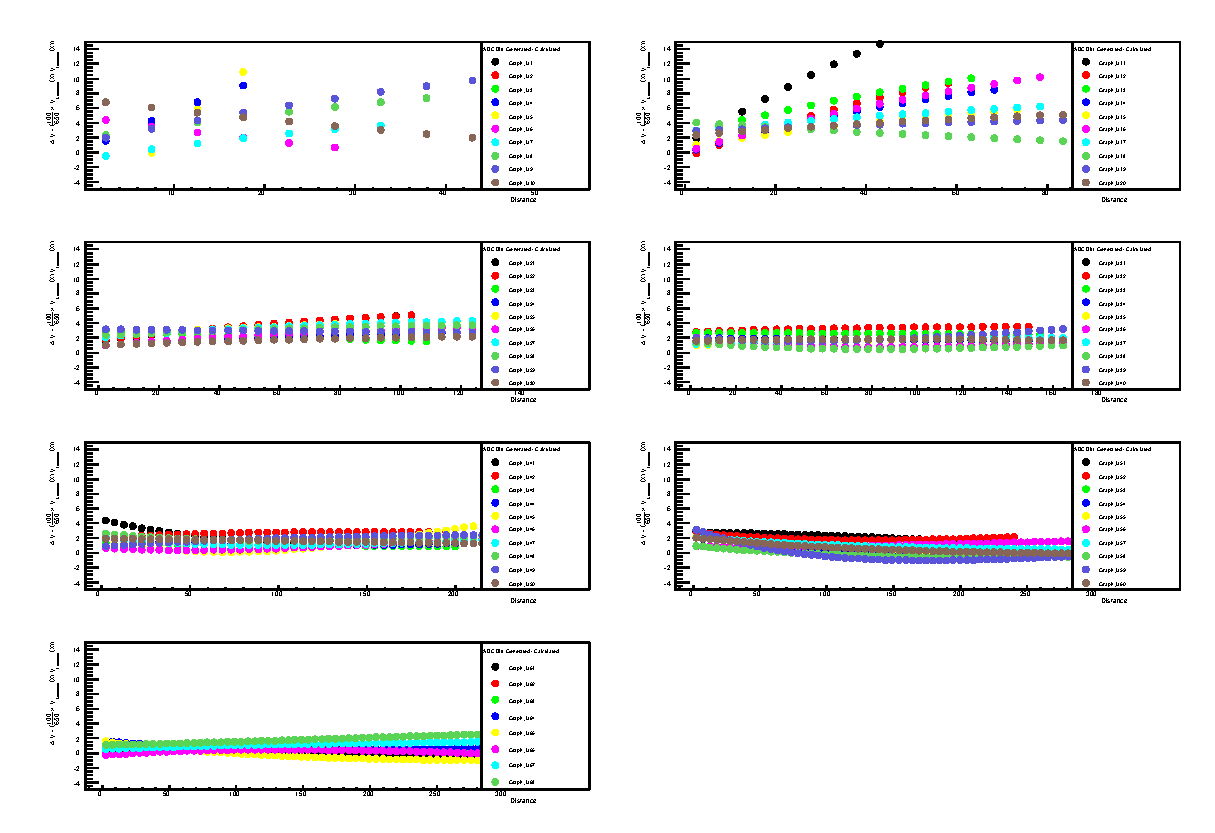
\includegraphics[width= 7in, keepaspectratio = true]{diffU}
\caption{Shown is the difference of the generated and calculated attenuation curves as a function of distance for all U-strips}
\label{fig:compGenCalcU}
\end{figure}

\begin{figure}[h]
\centering
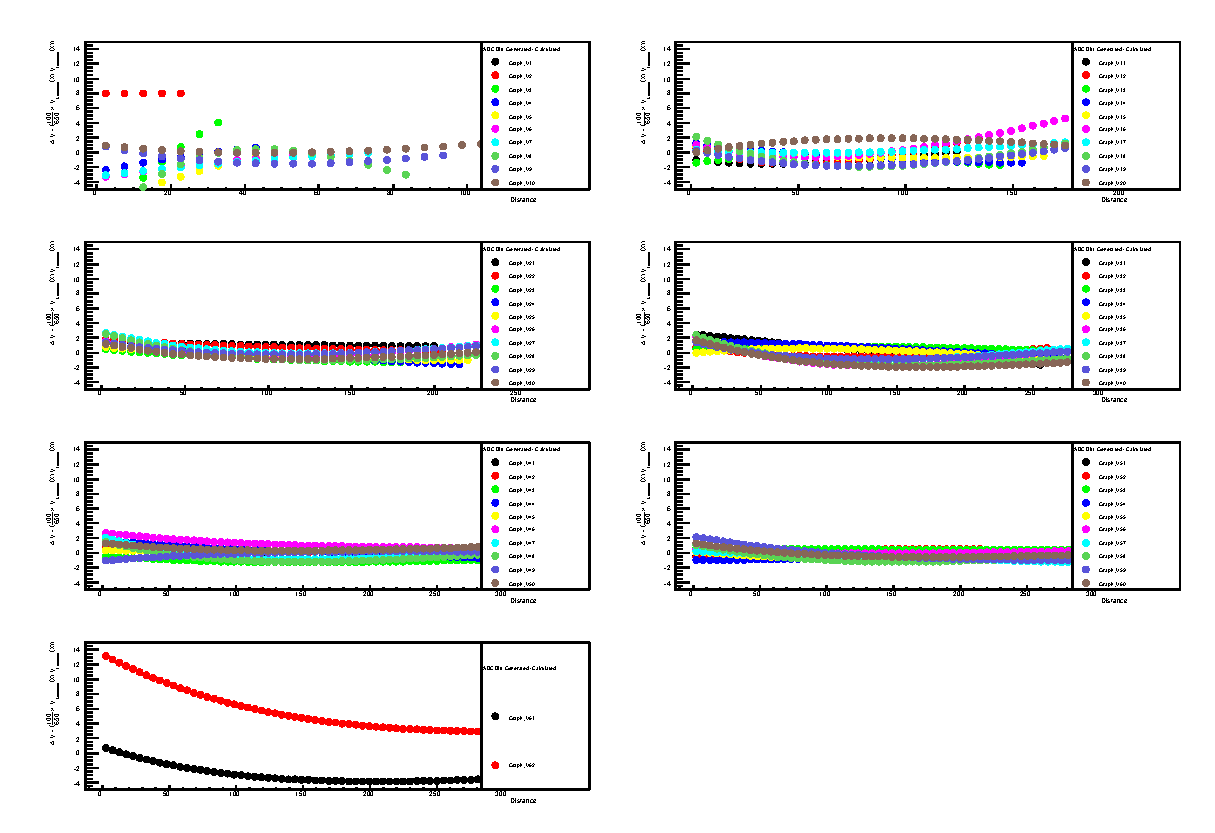
\includegraphics[width= 6in, keepaspectratio = true]{diffV}
\caption{Shown is the difference of the generated and calculated attenuation curves as a function of distance for all V-strips}
\label{fig:compGenCalcV}
\end{figure}

\begin{figure}[h]
\centering
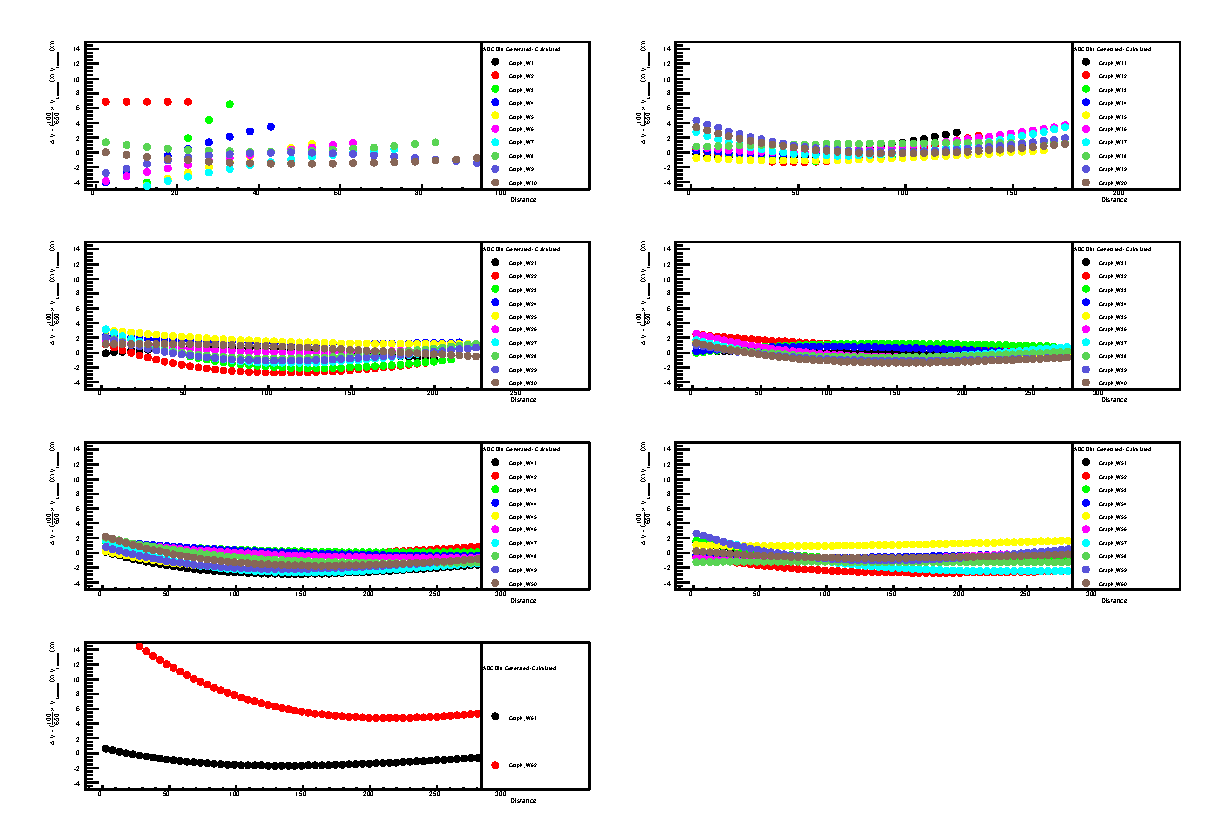
\includegraphics[width= 6in, keepaspectratio = true]{diffW}
\caption{Shown is the difference of the generated and calculated attenuation curves as a function of distance for all W-strips}
\label{fig:compGenCalcW}
\end{figure}
\FloatBarrier

\FloatBarrier
\subsection{With Iteration}
Another way to test the extracted calibration constants with respect to the generated coefficients is to compare
results with and without iterations. The iterations are explained in Section~\ref{Sec:fitToADCOutput}.  Figures~\ref{fig:diffU}-\ref{fig:diffW}
 show the comparison. The plots on the left are without iterations while those on the right correspond to the 
 coefficients produced from iterations. Comparisons of few longer strips for each view are only shown. The iterations are capable of
 reclaiming bad initial fits.
\begin{figure}[h]
    \centering
    \begin{subfigure}[h]{0.44\textwidth}
        \centering
        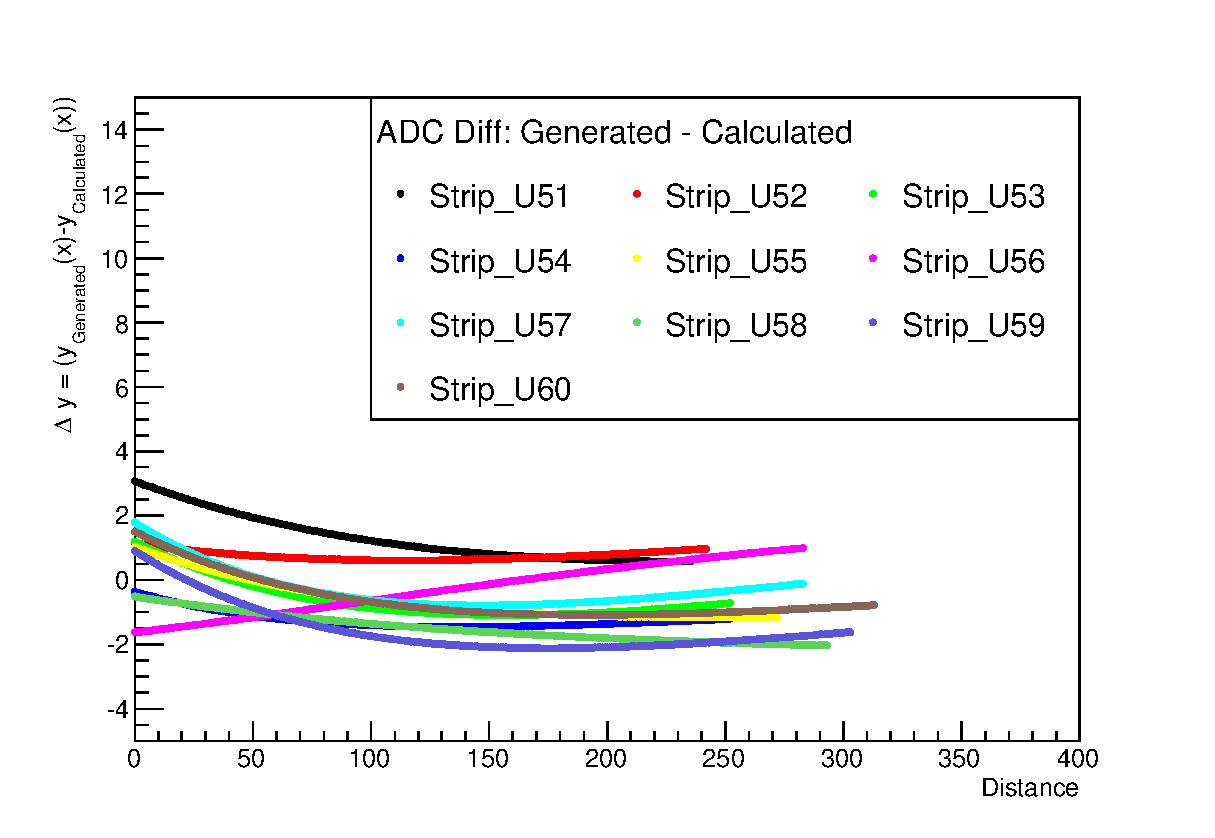
\includegraphics[width=\textwidth, keepaspectratio = true]{diffUMean_6}
        \caption{diffU6mean}
        \label{fig:diffU6mean}
    \end{subfigure}
    ~
    \begin{subfigure}[h]{0.44\textwidth}
        \centering
        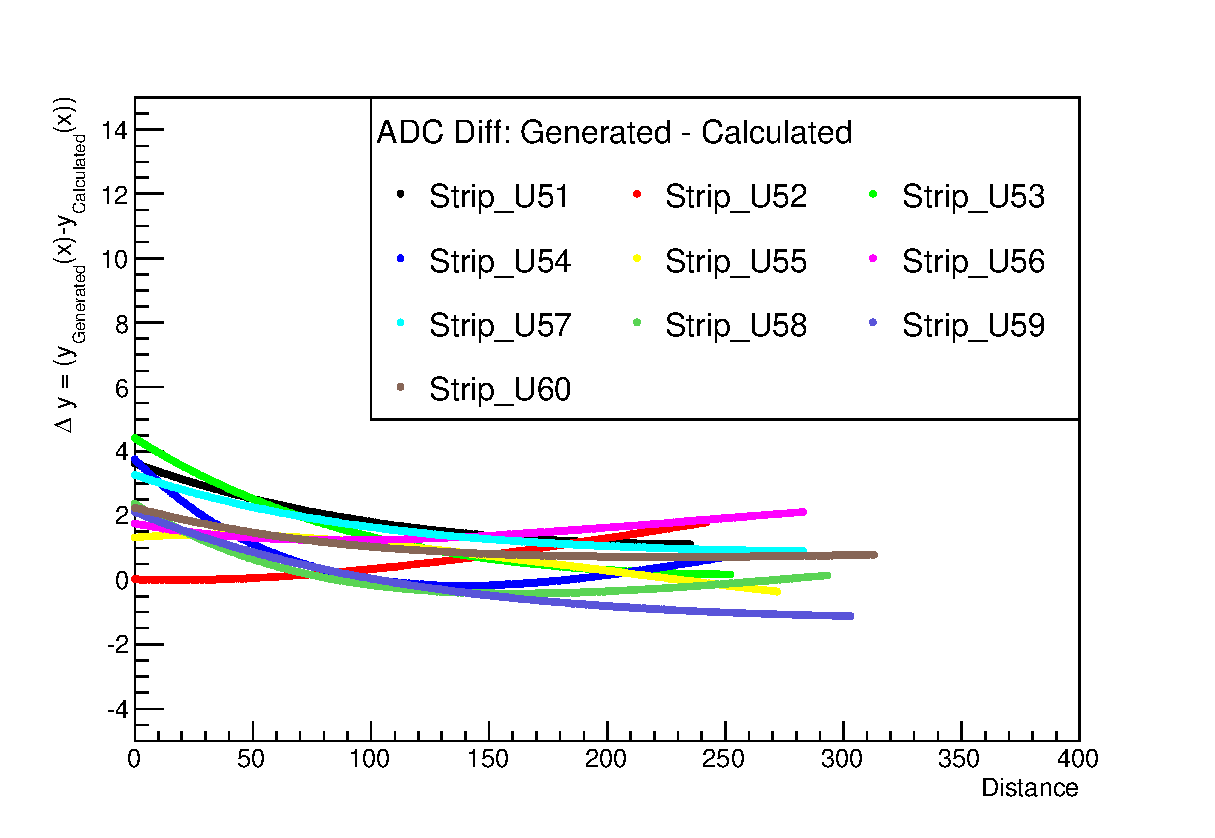
\includegraphics[width=\textwidth, keepaspectratio = true]{diffURoot_6}
        \caption{diffU6root}
        \label{fig:diffU6root}
    \end{subfigure}
    
    \begin{subfigure}[h]{0.44\textwidth}
        \centering
        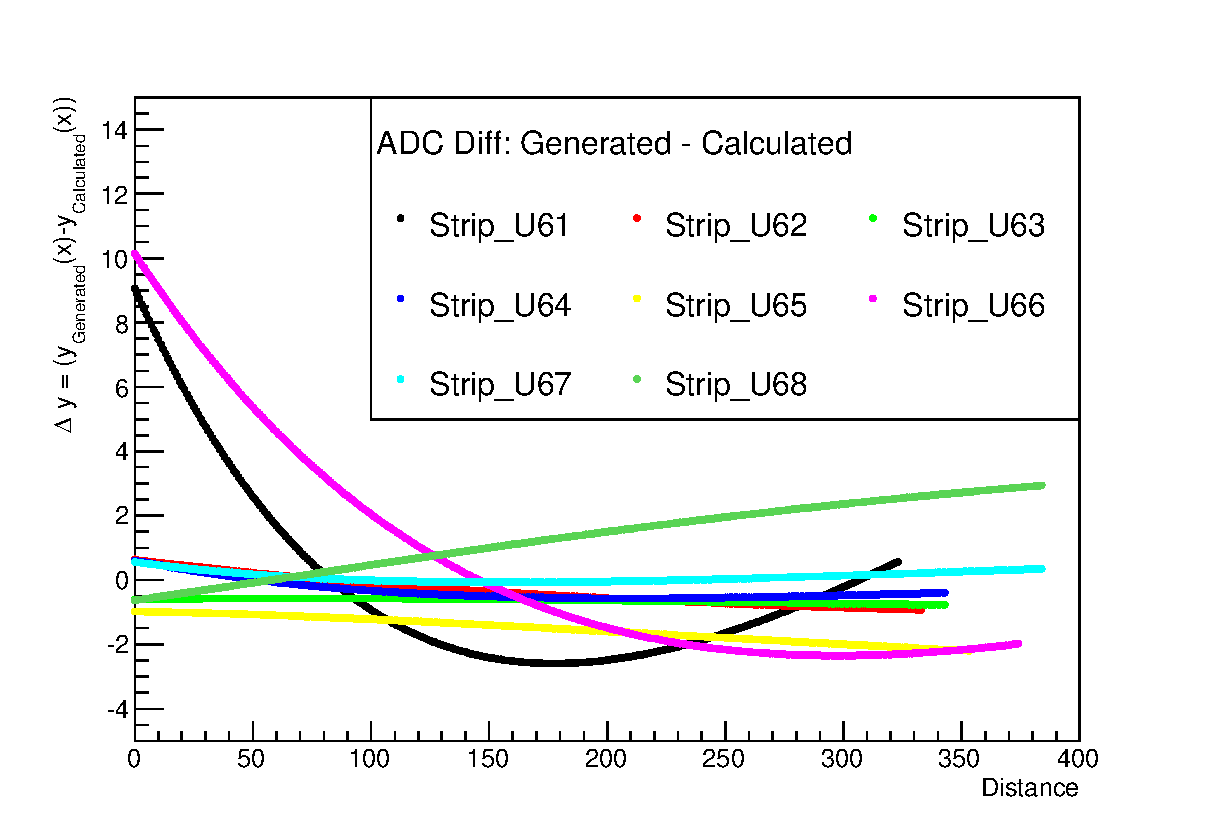
\includegraphics[width=\textwidth, keepaspectratio = true]{diffUMean_7}
        \caption{diffU7mean}
        \label{fig:diffU7mean}
    \end{subfigure}
    ~
    \begin{subfigure}[h]{0.44\textwidth}
        \centering
        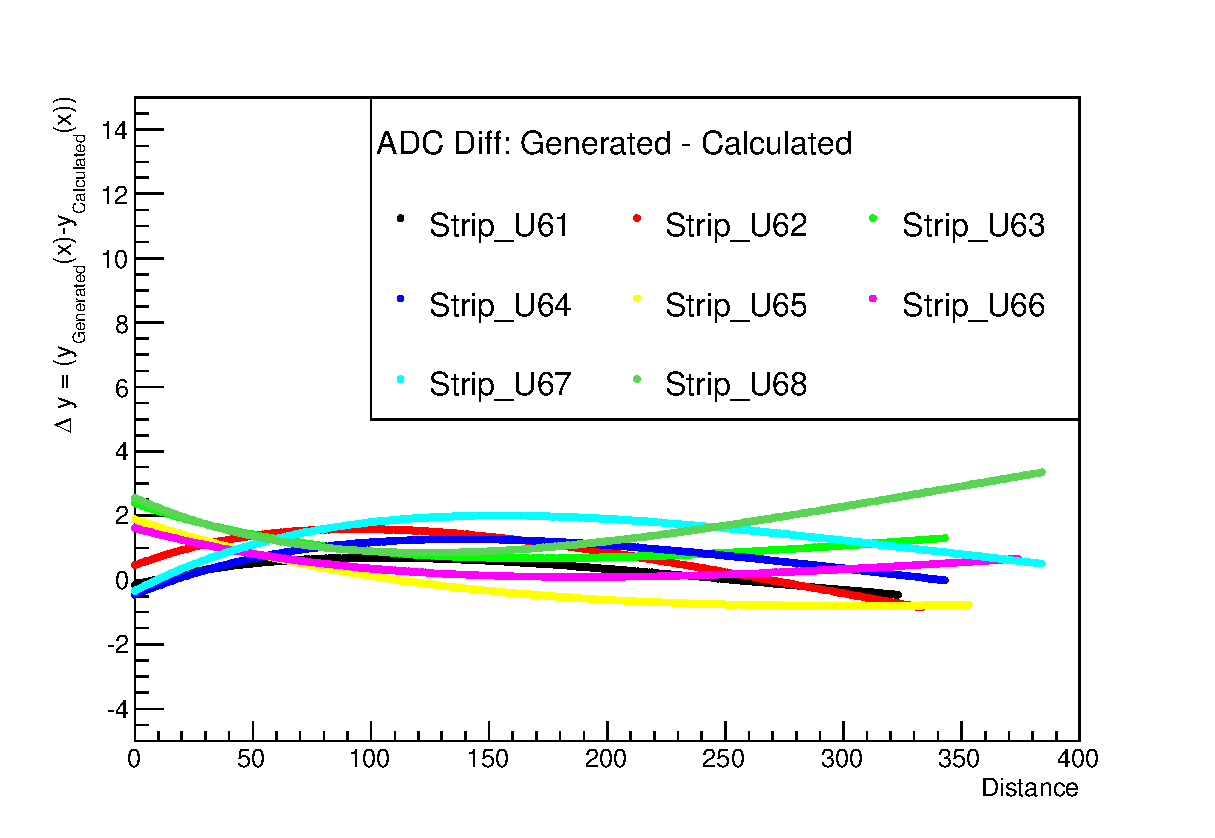
\includegraphics[width=\textwidth, keepaspectratio = true]{diffURoot_7}
        \caption{diffU7root}
        \label{fig:diffU7root}
    \end{subfigure}
    \caption{The plots on the left are based on coefficients extracted without any iteration while those on the right correspond to with 
    iterations. U-strips 51-68 are compared.}
    \label{fig:diffU}
\end{figure}
    
\begin{figure}[h]
    \centering
    \begin{subfigure}[h]{0.44\textwidth}
        \centering
        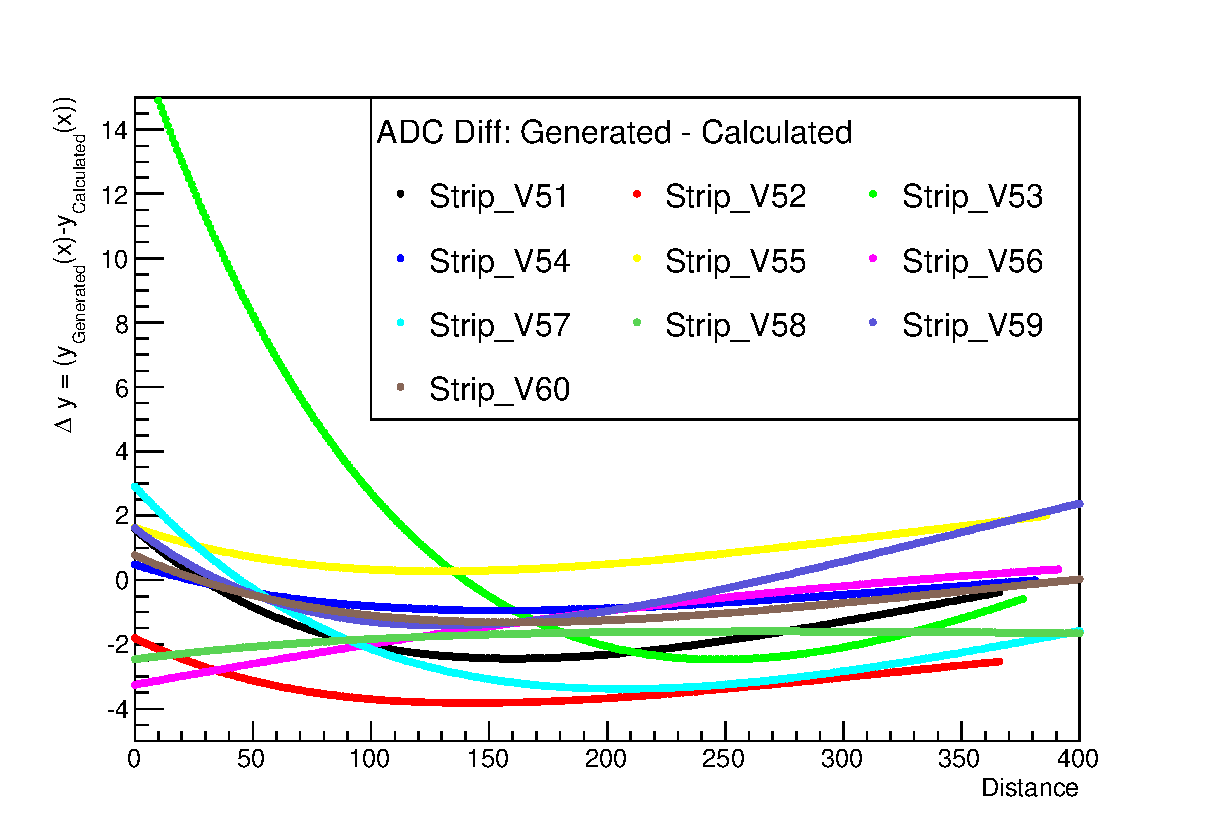
\includegraphics[width=\textwidth, keepaspectratio = true]{diffVMean_6}
        \caption{diffV6mean}
        \label{fig:diffV6mean}
    \end{subfigure}
    ~
    \begin{subfigure}[h]{0.44\textwidth}
        \centering
        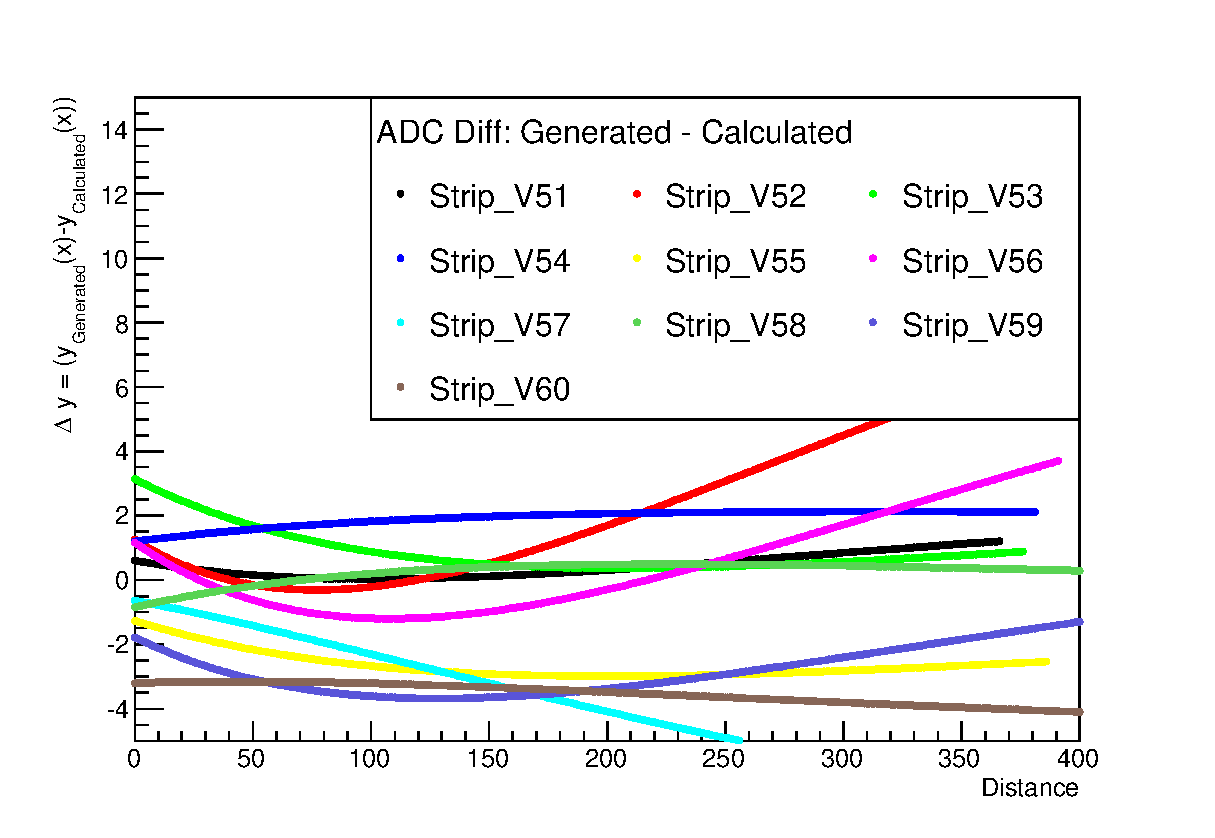
\includegraphics[width=\textwidth, keepaspectratio = true]{diffVRoot_6}
        \caption{diffV6root}
        \label{fig:diffV6root}
    \end{subfigure}
    
    \begin{subfigure}[h]{0.44\textwidth}
        \centering
        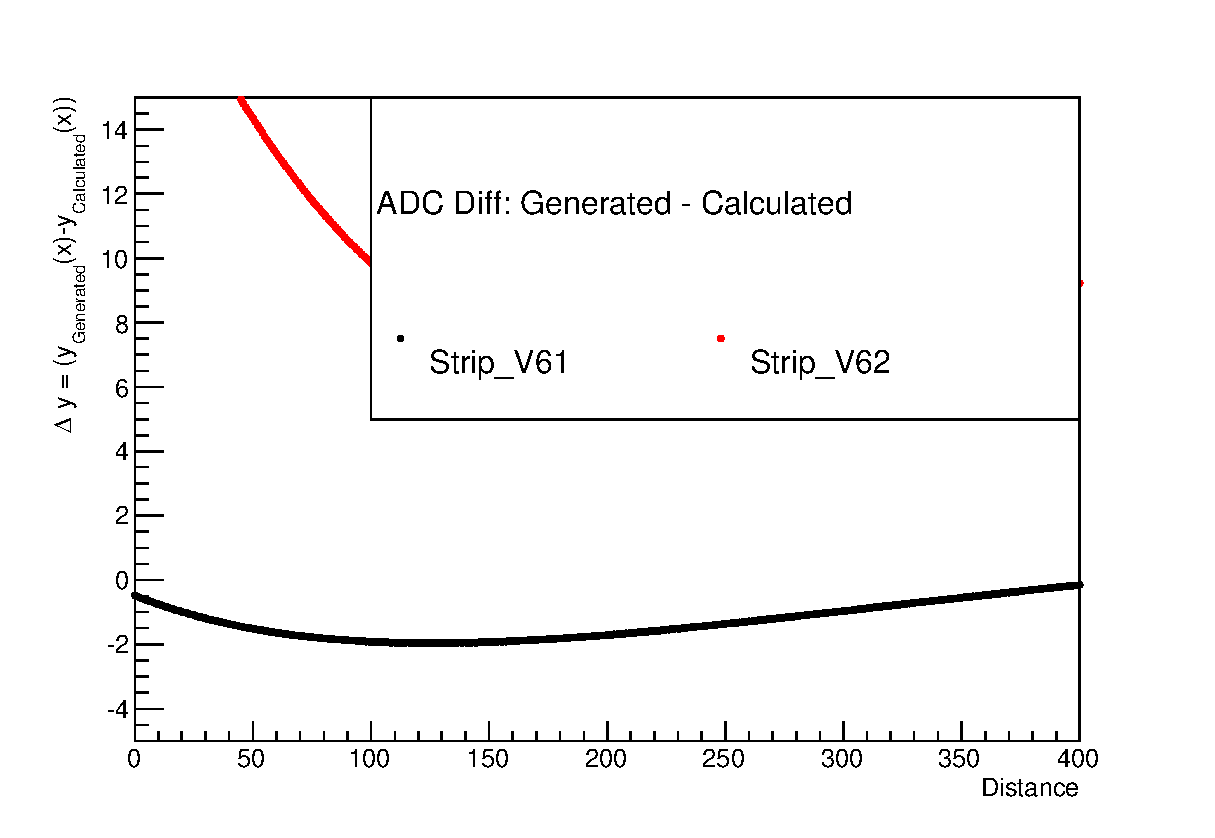
\includegraphics[width=\textwidth, keepaspectratio = true]{diffVMean_7}
        \caption{diffV7mean}
        \label{fig:diffV7mean}
    \end{subfigure}
    ~
    \begin{subfigure}[h]{0.44\textwidth}
        \centering
        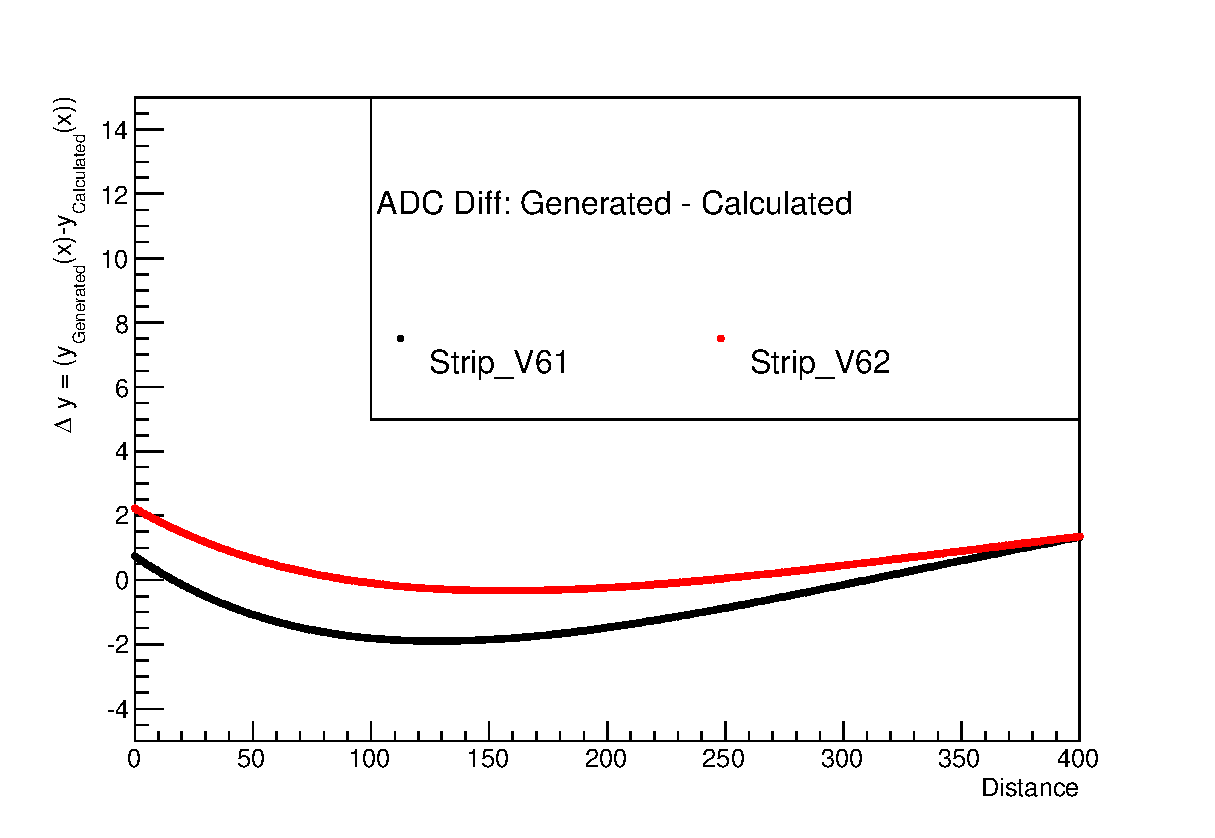
\includegraphics[width=\textwidth, keepaspectratio = true]{diffVRoot_7}
        \caption{diffV7root}
        \label{fig:diffV7root}
    \end{subfigure}
    \caption{The plots on the left are based on coefficients extracted without any iteration while those on the right correspond to with 
    iterations. V-strips 51-62 are compared.}
    \label{fig:diffV}
\end{figure}

\begin{figure}[h]
    \centering
    \begin{subfigure}[h]{0.44\textwidth}
        \centering
        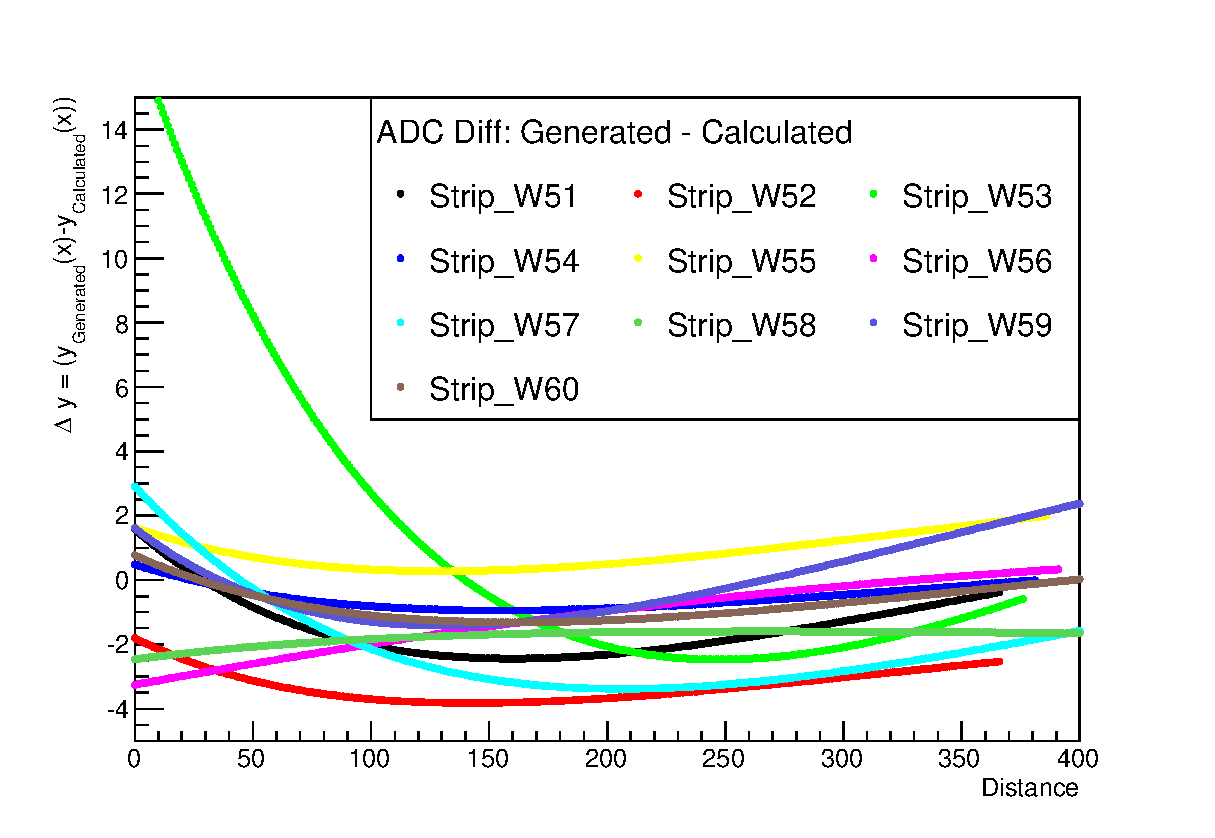
\includegraphics[width=\textwidth, keepaspectratio = true]{diffWMean_6}
        \caption{diffW6mean}
        \label{fig:diffW6mean}
    \end{subfigure}
    ~
    \begin{subfigure}[h]{0.44\textwidth}
        \centering
        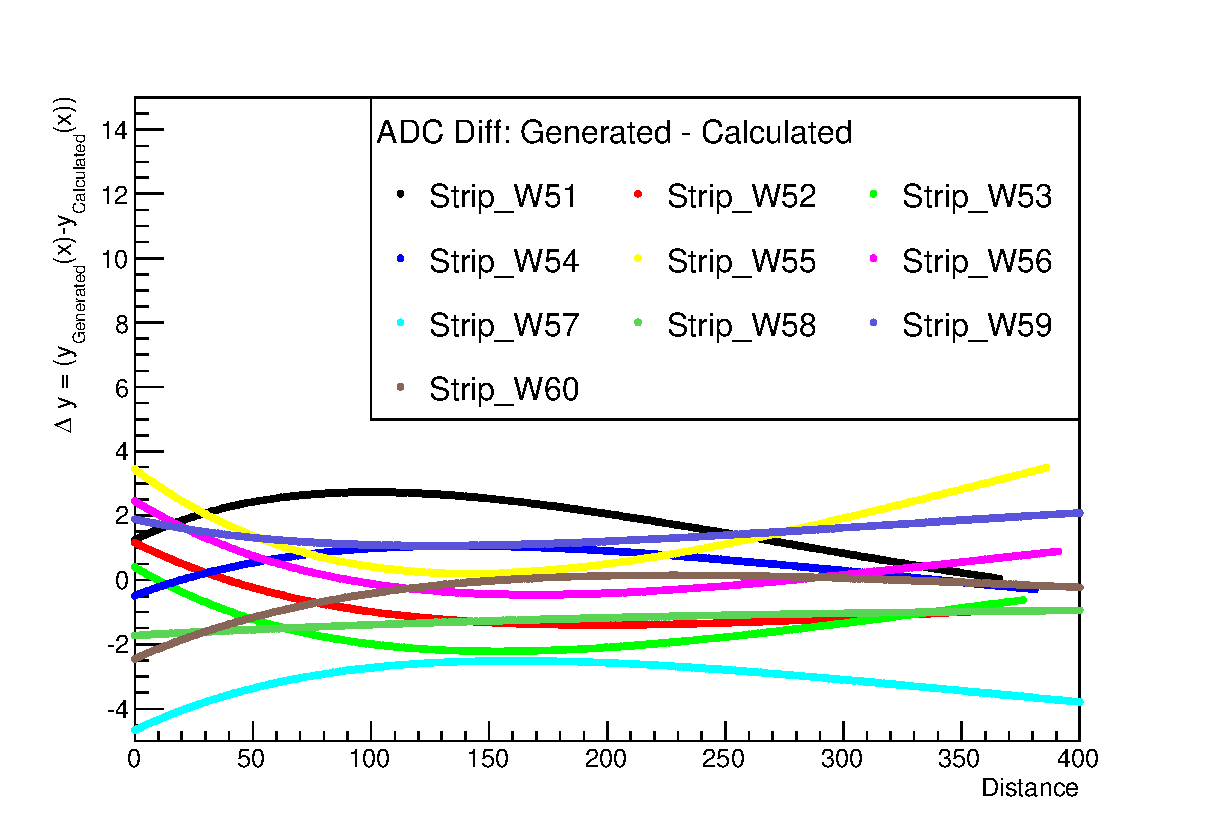
\includegraphics[width=\textwidth, keepaspectratio = true]{diffWRoot_6}
        \caption{diffW6root}
        \label{fig:diffW6root}
    \end{subfigure}
    
    \begin{subfigure}[h]{0.44\textwidth}
        \centering
        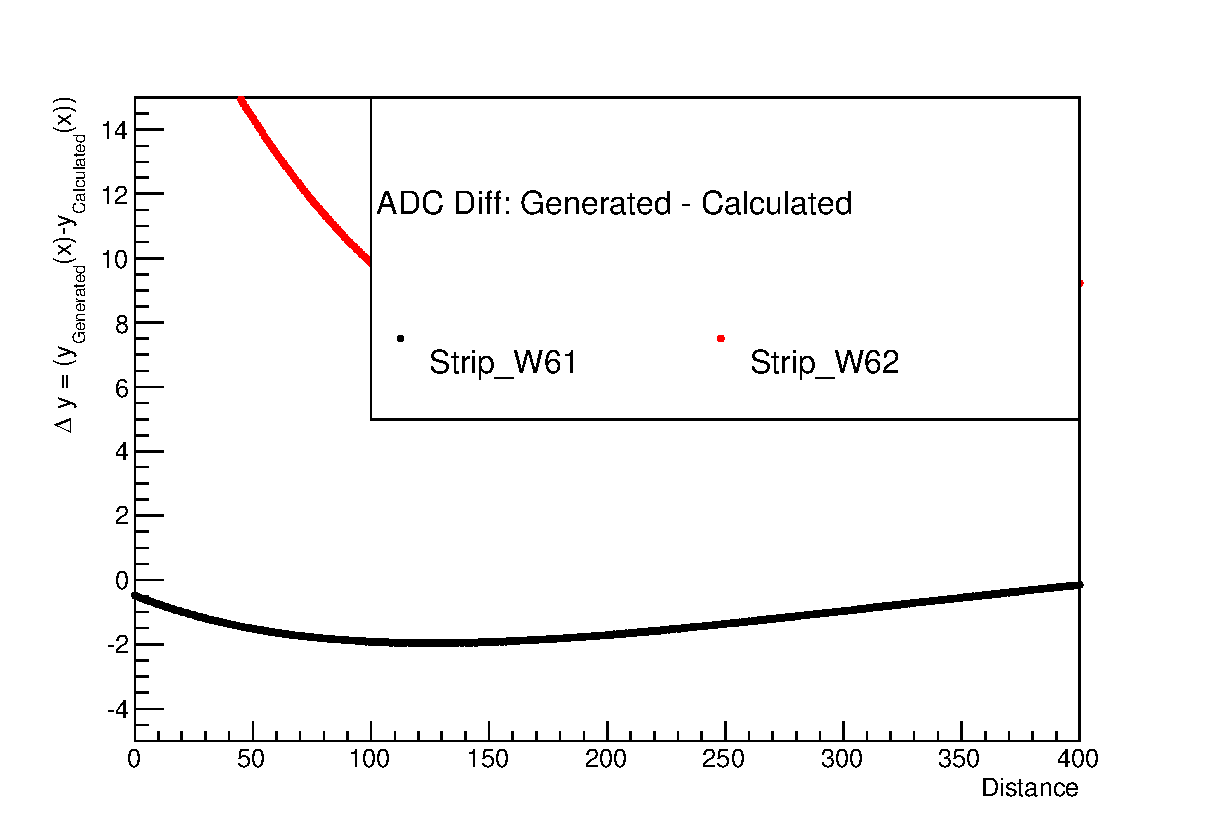
\includegraphics[width=\textwidth, keepaspectratio = true]{diffWMean_7}
        \caption{diffW7mean}
        \label{fig:diffW7mean}
    \end{subfigure}
    ~
    \begin{subfigure}[h]{0.44\textwidth}
        \centering
        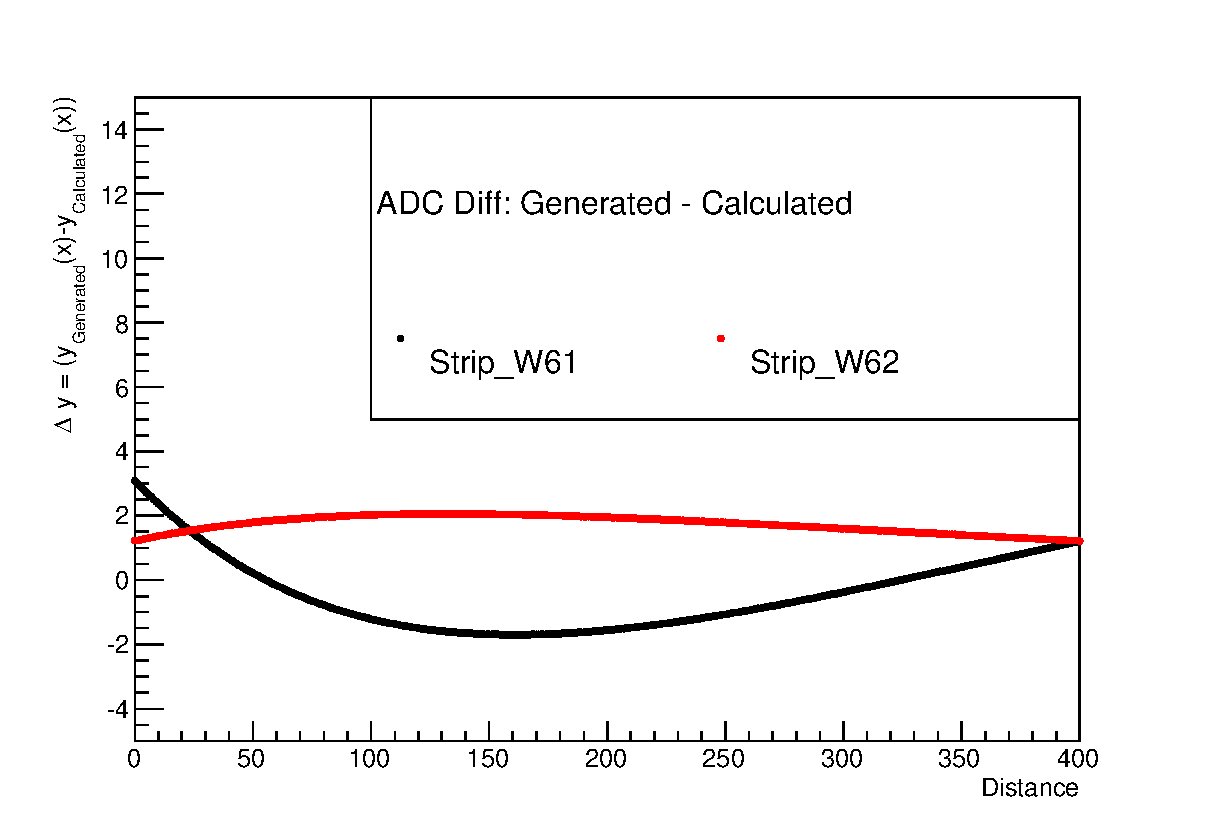
\includegraphics[width=\textwidth, keepaspectratio = true]{diffWRoot_7}
        \caption{diffW7root}
        \label{fig:diffW7root}
    \end{subfigure}
    \caption{The plots on the left are based on coefficients extracted without any iteration while those on the right correspond to with 
    iterations. W-strips 51-62 are compared.}
    \label{fig:diffW}
\end{figure}
\FloatBarrier
%\section{Acceptance}
